\chapter{ANÁLISIS Y DISCUSIÓN DE RESULTADOS}
\section{Metadata}
Luego de 27 épocas, con un rango entre 2 y 3 segundos de entrenamiento cada una, el modelo dejó de entrenar dado que durante 7 épocas no registró una reducción en el valor de la pérdida del subconjunto de validación, por más que 3 épocas antes se había reducido su tasa de aprendizaje.

Así, de acuerdo a las Figuras \ref{5:fig1} y \ref{5:fig2}, en la época 20 se registran los mejores valores de exactitud y pérdida para el subconjunto de validación, alcanzando 0.9523 y 0.1246 respectivamente.

\begin{figure}[htbp]
	\begin{center}
		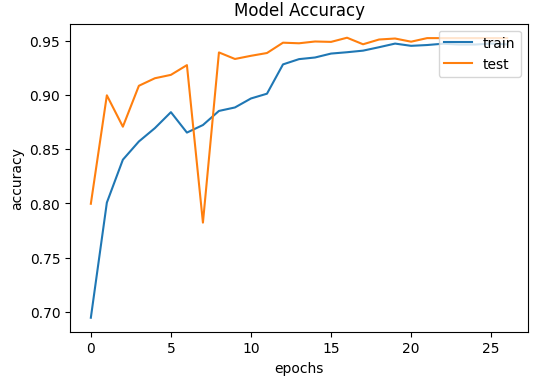
\includegraphics[width=0.60\textwidth]{4/figures/metadata_model_accuracy.png}
		\caption{Evolución de la exactitud de los subconjuntos de entrenamiento y validación para el modelo MLP de metadata para un entrenamiento de 100 épocas. Fuente: Elaboración propia.}
		\label{5:fig1}
		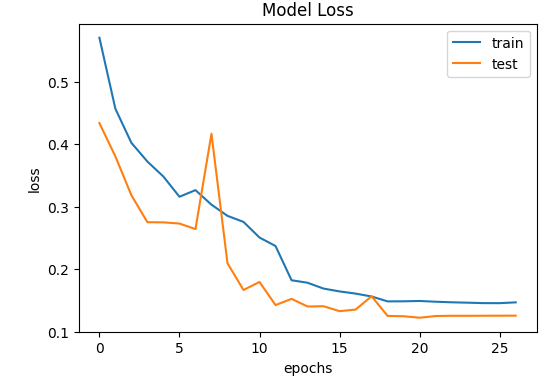
\includegraphics[width=0.60\textwidth]{4/figures/metadata_model_loss.png}
		\caption{Evolución de la pérdida de los subconjuntos de entrenamiento y validación para el modelo MLP de metadata para un entrenamiento de 100 épocas. Fuente: Elaboración propia.}
		\label{5:fig2}
	\end{center}
\end{figure}

La matriz de confusión resultante se representa en la Figura \ref{5:fig3}.

\begin{figure}[!ht]
	\begin{center}
		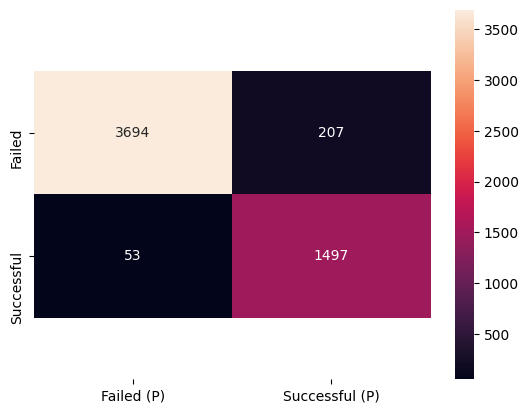
\includegraphics[width=0.60\textwidth]{4/figures/metadata_confusion_matrix.png}
		\caption{Matriz de confusión para el modelo MLP de metadata. Fuente: Elaboración propia.}
		\label{5:fig3}
	\end{center}
\end{figure}

De esta matriz, derivan los siguientes resultados evaluados según las métricas seleccionadas (citar).

\section{Descripción}
Luego de 78 épocas, con un rango entre 102 y 114 segundos de entrenamiento cada una, el modelo dejó de entrenar dado que durante 10 épocas no registró una reducción en el valor de la pérdida del subconjunto de validación, por más que 5 épocas antes se había reducido su tasa de aprendizaje.

Así, de acuerdo a las Figuras \ref{5:fig4} y \ref{5:fig5}, en la época 68 se registran los mejores valores de exactitud y pérdida para el subconjunto de validación, alcanzando 0.7665 y 0.4922 respectivamente.

\begin{figure}[htbp]
	\begin{center}
		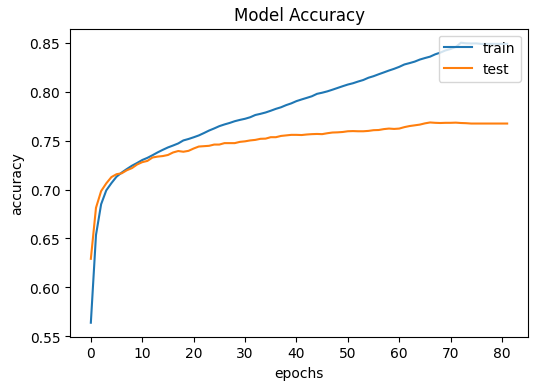
\includegraphics[width=0.60\textwidth]{4/figures/description_model_accuracy.png}
		\caption{Evolución de la exactitud de los subconjuntos de entrenamiento y validación para el modelo CNN de descripciones para un entrenamiento de 100 épocas. Fuente: Elaboración propia.}
		\label{5:fig4}
		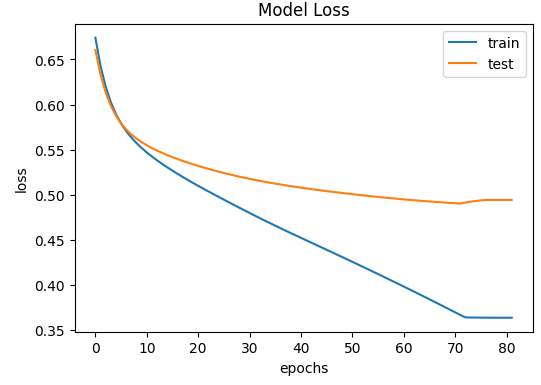
\includegraphics[width=0.60\textwidth]{4/figures/description_model_loss.png}
		\caption{Evolución de la pérdida de los subconjuntos de entrenamiento y validación para el modelo CNN de descripciones para un entrenamiento de 100 épocas. Fuente: Elaboración propia.}
		\label{5:fig5}
	\end{center}
\end{figure}

La matriz de confusión resultante se representa en la Figura \ref{5:fig6}.

\begin{figure}[!ht]
	\begin{center}
		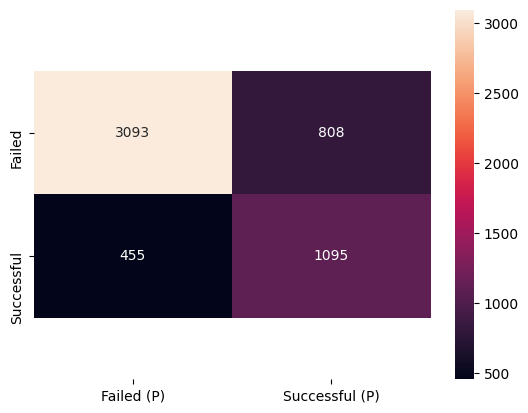
\includegraphics[width=0.60\textwidth]{4/figures/description_confusion_matrix.png}
		\caption{Matriz de confusión para el modelo CNN de descripciones. Fuente: Elaboración propia.}
		\label{5:fig6}
	\end{center}
\end{figure}

De esta matriz, derivan los siguientes resultados evaluados según las métricas seleccionadas (citar).

\section{Comentarios}

